\documentclass[14pt]{extarticle}
\usepackage{fontspec}
\usepackage[dvipsnames]{xcolor}
\usepackage{titlesec}
\usepackage[left=1.8cm,right=2.0cm,top=0.75cm,bottom=0.75cm,headheight=17pt,headsep=0.5cm,includehead,includefoot]{geometry}
\usepackage{fancyhdr}
\usepackage{graphicx}
\usepackage{background}
\usepackage{zref-savepos}
\usepackage[colorlinks,
linkcolor={red!50!black},
citecolor={blue!50!black},
urlcolor={blue!80!black}]{hyperref}
\usepackage{subcaption}
\usepackage{float}
\usepackage{tabularx}
\usepackage[framemethod=TikZ]{mdframed}
\usepackage{parskip}
\usepackage{pgfgantt}
\usepackage{multicol}

\setmainfont{Equity Text A}
\setsansfont{Concourse T3}
\setmonofont{Triplicate T4}
\renewcommand{\familydefault}{\sfdefault}
\newfontfamily\sectionfont{Concourse C3}

\titleformat{\section}{\sectionfont\Huge\selectfont\bfseries}{}{0pt}{}[]
\titlespacing{\section}{0cm}{2cm}{0.5cm}
\titleformat{\subsection}{\normalfont\large\bfseries}{}{0pt}{}

\pagestyle{fancy}
\fancyhf{}
\rhead{\textcolor{white}{\bfseries\rightmark}}
\lfoot{\textcolor{white}{\bfseries\thepage}}
\renewcommand{\sectionmark}[1]{\markright{#1}}
\renewcommand{\headrulewidth}{0pt}
\renewcommand{\subsectionmark}[1]{}
\captionsetup[subfigure]{labelformat=empty}

\definecolor{barblue}{RGB}{15,74,119}

\makeatletter
\def\@afterheading{%
  \@nobreaktrue
  \everypar{%
    \if@nobreak
    \@nobreakfalse
    \clubpenalty \@M
    \hspace*{1em}%
    \else
    \clubpenalty \@clubpenalty
    \everypar{}%
    \fi}}
\makeatother
\setlength{\parindent}{0pt}

\backgroundsetup{
  scale=1,
  color=black,
  opacity=1.0,
  angle=0
}

\newcommand{\coverpage}[1]{
  \clearpage
  \thispagestyle{empty}
  \SetBgContents{\includegraphics[width=\paperwidth,height=\paperheight]{#1}}
  \null
  \thispagestyle{empty}%
  \addtocounter{page}{-1}%
  \newpage
  \SetBgContents{\includegraphics[width=\paperwidth,height=\paperheight]{background}}
}

\newcommand{\fillgraphics}[2][]{%
  \par
  \zsaveposy{top-\thepage}% Mark (baseline of) top of image
  \vfill
  \zsaveposy{bottom-\thepage}% Mark (baseline of) bottom of image
  \smash{\includegraphics[height=\dimexpr\zposy{top-\thepage}sp-\zposy{bottom-\thepage}sp\relax,#1]{#2}}%
  \par
}

\newcommand{\includemovie}[2]{
  \begin{subfigure}[b]{0.3\textwidth}
    \begin{center}
      \href{https://raw.githubusercontent.com/Shinmera/kandria/master/doc/pitch/#1.gif}{\includegraphics[width=\textwidth]{#1}}
    \end{center}
    \caption{#2}
  \end{subfigure}
}

\newcolumntype{R}{>{\raggedleft\arraybackslash}X}
\newcommand\setrow[1]{\gdef\rowmac{#1}#1\ignorespaces}
\newcommand\clearrow{\global\let\rowmac\relax}
\clearrow

\begin{document}
\coverpage{cover.jpg}
\begin{figure}[H]
  \centering
  \vspace{-1.5cm}
  \advance\leftskip-1.8cm
  \includegraphics[width=\pagewidth]{../media/library hero.png}
\end{figure}

\section{About Kandria}
Kandria is a hack and slash, puzzle platforming game set in a broken down, post-apocalyptic desert.

You play a lone android, who must help a struggling settlement survive. Travel far and wide, taking on missions for whomever you choose - explore the ruined surface, scale steep cliffs, or venture deep below ground to gather supplies and long-buried relics. Show off your combat skills by slashing your way through any opposition in a flurry of extravagant sword moves. As an android there is no limit to where you can go or what you can do.

As the story unfolds you’ll get to know the flawed and diverse characters of the settlement that rescued you. But are they really your friends, or are you just their tool? On your travels you must determine who is truly friend or foe, and recruit what allies you can - because the end is coming.

%%% Local Variables:
%%% mode: latex
%%% TeX-master: "pitch"
%%% TeX-engine: luatex
%%% End:

\section{Current Status}
We are currently nearing the end of the vertical slice development, which spans most of the first act of the game's story. In order to do this, we've built complex quest and dialogue systems, as well as intricate platforming and combat mechanics. The slice also features most of the main cast of characters, as well as two distinct and detailed environments.

\begin{figure}[h]
  \centering
  \begin{subfigure}[b]{0.60\textwidth}
    \centering
    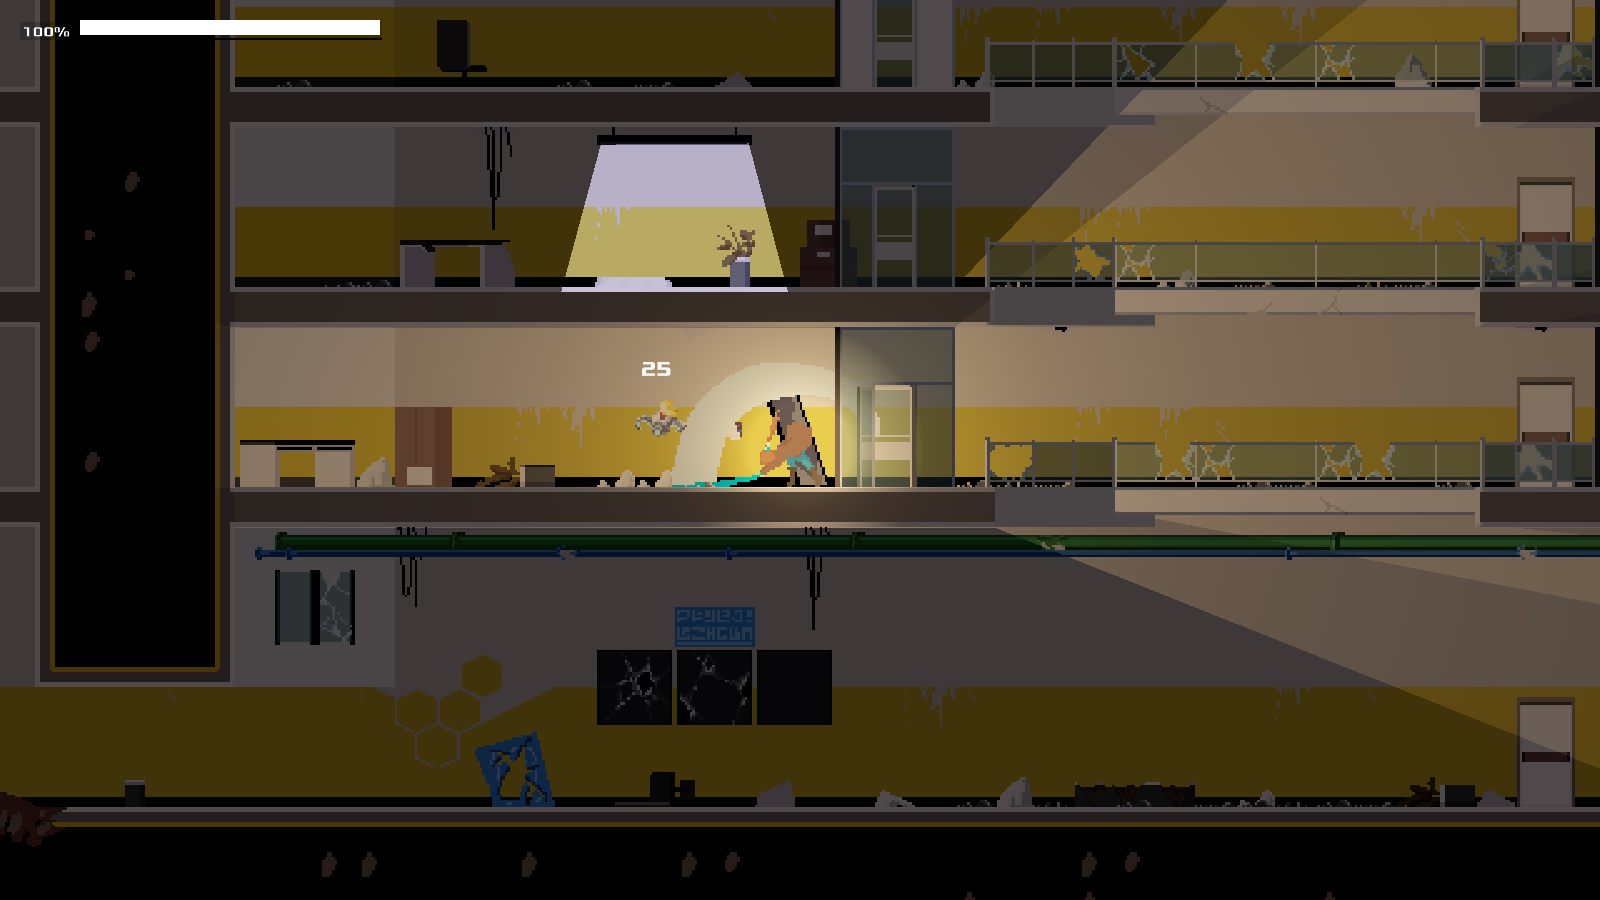
\includegraphics[width=\textwidth]{../press/screenshot 1.png}
  \end{subfigure}
  \begin{subfigure}[b]{0.35\textwidth}
    \centering
    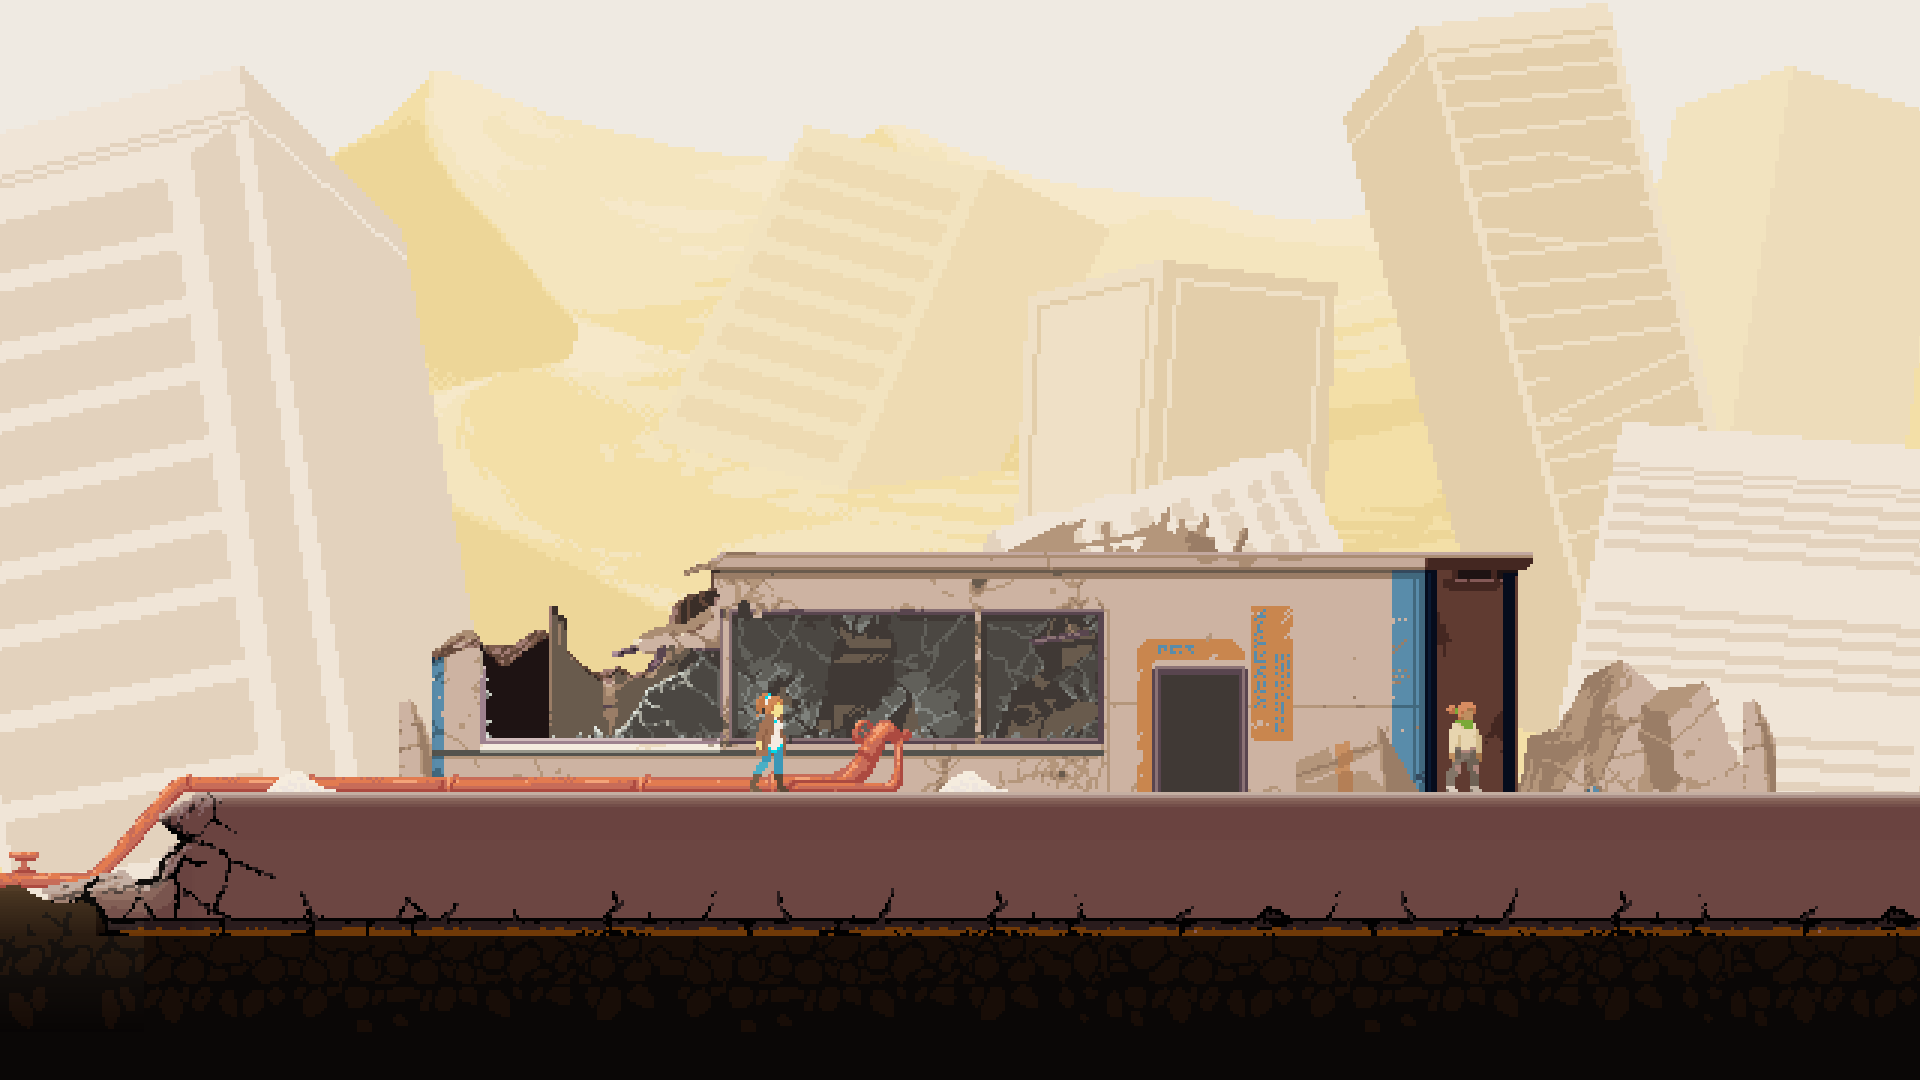
\includegraphics[width=\textwidth]{../press/screenshot 8.png}
  \end{subfigure}
  \vskip -0.5cm
  \begin{subfigure}[t]{0.35\textwidth}\vskip 0pt
    \centering
    \includegraphics[width=\textwidth]{../press/screenshot 2.png}
  \end{subfigure}
  \begin{subfigure}[t]{0.55\textwidth}\vskip 0pt
    \centering
    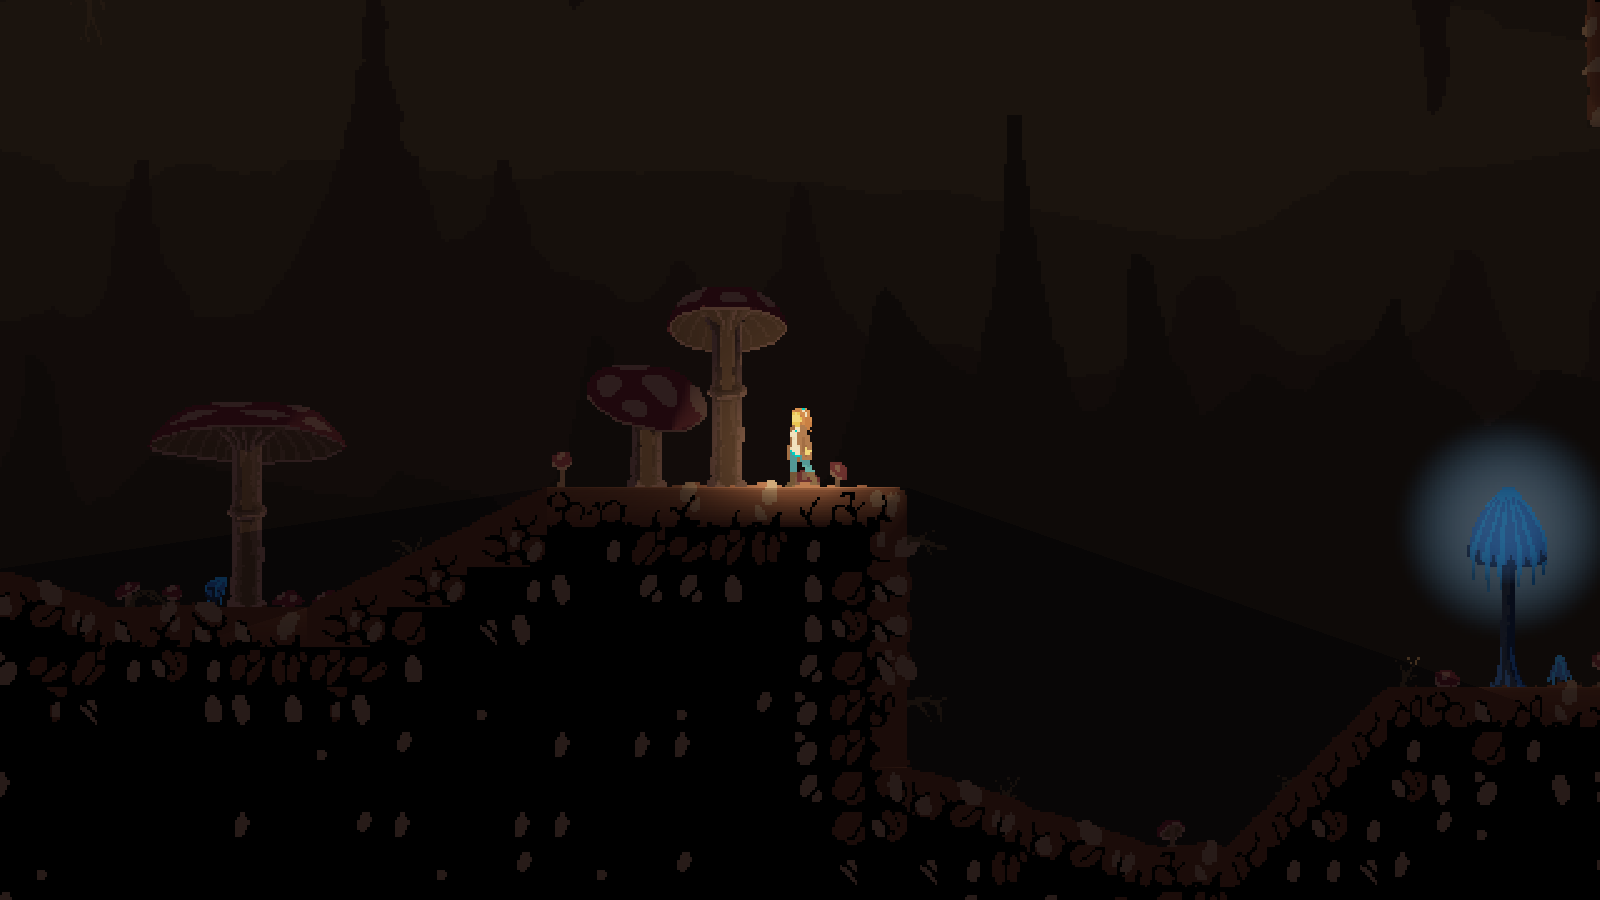
\includegraphics[width=\textwidth]{../press/screenshot 3.png}
  \end{subfigure}
\end{figure}

Having spent a good chunk of pre-production and the slice development on figuring out our process and developing our tools, we can now produce content with much more confidence and efficiency. Most of the required systems for the full game are in place and working well, too, so we can focus more on the design.

We've also written detailed design documents describing the \href{https://kandria.com/lore}{setting}, \href{https://kandria.com/plot outline}{story}, \href{https://kandria.com/characters}{characters}, \href{https://kandria.com/art}{visuals}, and so forth in order to create a cohesive narrative and world for the player to explore.

\clearpage
\subsection{Story and World}
Kandria's world is set in the not too distant future. Humanity has built massive, glistening cities on earth's surface, and deep webs of tunnels and complexes underground. Most of the manufacturing process is automated now, even down to primitive humanoid robots... or at least so you would be led to believe if you enjoy a life of comfort on the surface. Underground the situation was very different. People were used primarily as an exploited workforce, either to maintain and manage the systems used above, or to mine and process rare materials.

Around this time, true AI was finally discovered. By a process that was not fully understood, devices could be manufactured that would learn and interpret information like a real brain. It didn't take long before this technology was incorporated into a humanoid chassis, birthing the first true android. This posed another vital step in the progress of fully automating all of human civilisation. However, shortly after the first few androids were developed in the field, calamity struck.

\begin{figure}[h]
  \centering
  \includegraphics[width=\textwidth]{../press/screenshot 6.png}
\end{figure}

The surface world was almost entirely wiped out, cities flattened and ground into dust with only ruins and deserts left in their wake. Many of the underground tunnels and structures collapsed, and humanity was brought to the brink of extinction. Only few survived underground, and with the catastrophe in mind, became reclusive and protective.

\clearpage
\begin{figure}[h]
  \centering
  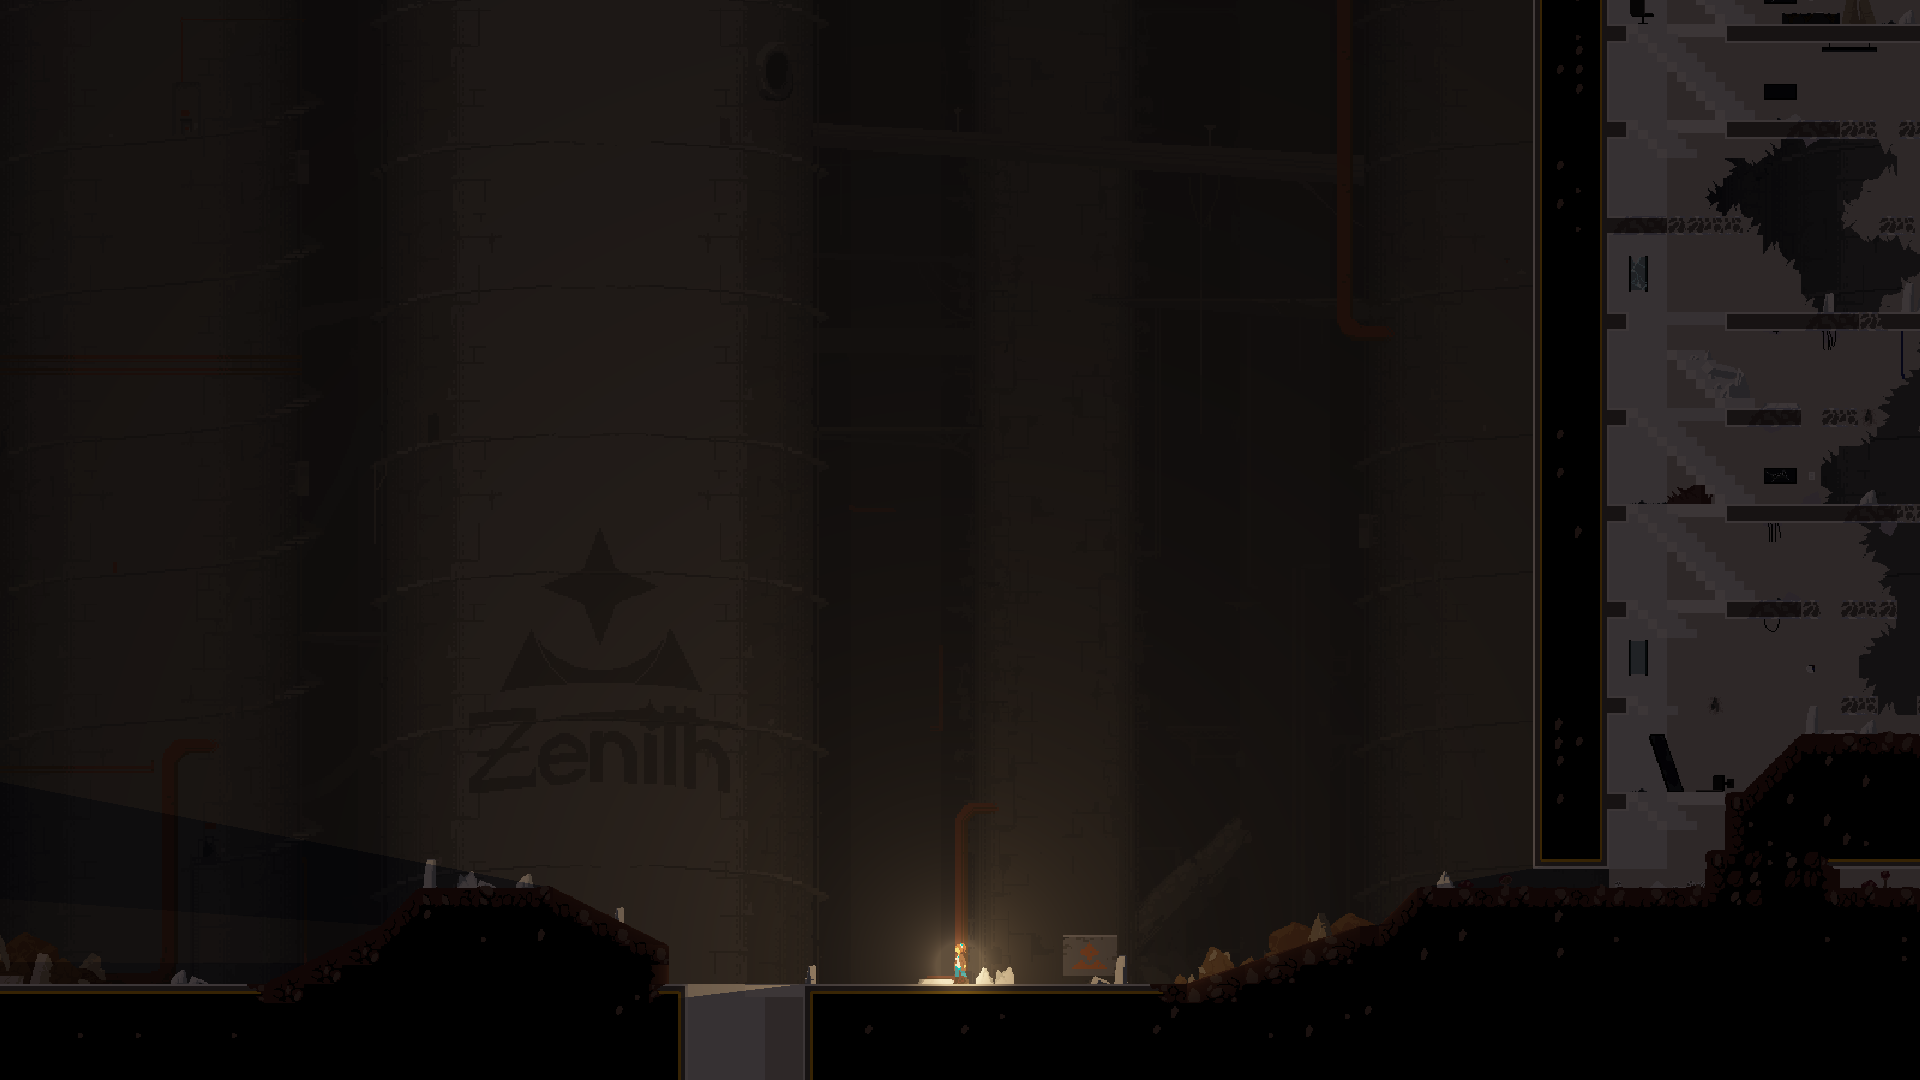
\includegraphics[width=\textwidth]{../press/screenshot 9.png}
\end{figure}

The game begins a few decades after the calamity, set in the valley of the former city of Zenith -- the underground areas now controlled by a few distinct factions, with raiders and other outcast groups roaming the tunnels and abandoned sites. One of those factions is undergoing internal conflict, a violent and militaristic group is struggling for power. Worried by this turn of events, and having discovered an old-world seed cache, Fi and her closest friends decide to separate and attempt to build their own faction back on the abandoned surface.

Near this seed cache they discover the slumbering remains of an android -- you -- and manage to reactivate it. Now back on your feet, with all of your memories lost to a data corruption, it's up to you to decide what to do. Will you follow after them or forge your own path?

Exploring the underground you'll come across other factions, each with their own values and beliefs, their own ideas on how to recover from this catastrophe. It is now up to you to earn their trust and defend what you hold dear from the harsh world. No matter what you do though, the conflict in Fi's home faction is reaching its boiling point, and will inevitably affect everyone else in the valley.

%%% Local Variables:
%%% mode: latex
%%% TeX-master: "pitch"
%%% TeX-engine: luatex
%%% End:

\section{Future Development}\label{sec:future}
We are nearing the completion of the vertical slice. This has given us a good idea on the required effort for a large section of the game. As a next step we are intending on completing the first half of the first act of the game, which includes the game's introduction and tutorial. In order to do so we'll also have to further polish and refine the existing mechanics and assets, and develop the first few custom music tracks.

This first half can then be used as marketing material by publishing it on Steam as a free ``First Act Demo''. This should help grow our community and gather general interest in the project. We can further use the demo as pitching material for grant applications and other investment opportunities.

From there the plan is to develop a horizontal slice -- laying out all the areas and story beats in broad strokes, to give us a better idea of the overall length of the game and its flow. We are aiming for a 10-12 hour playtime in total, and putting together the horizontal slice should give us a much better idea of how much content we can cut or have to expand on. It should also help a lot to settle the overall story structure and build towards a pleasing tension arc.

After the slice is completed and tested, we can then move on to fleshing it out, chapter by chapter, building up to a complete product. Finally, the last half year should be spent testing, polishing, and refining the game to make it as good as can be.

\subsection{Investment Use}
Money from investment would primarily be put to use to avoid having to cut features from the game and to expand its budget for music, sound, and ultimately marketing, which should help a lot to increase the value of the game and ensure its success.

%%% Local Variables:
%%% mode: latex
%%% TeX-master: "pitch"
%%% TeX-engine: luatex
%%% End:

\section{Team}
The team for Kandria currently consists of three core members.

\begin{figure}[h]
  \centering
  \begin{subfigure}[t]{0.3\textwidth}
    \centering
    \includegraphics[width=4cm]{nicolas.png}
    \caption{\centering\textbf{Nicolas Hafner}\\Producer, programmer, artist, designer}
  \end{subfigure}
  \begin{subfigure}[t]{0.3\textwidth}
    \centering
    \includegraphics[width=4cm]{tim.png}
    \caption{\centering\textbf{Tim White}\\Writer, designer}
  \end{subfigure}
  \begin{subfigure}[t]{0.3\textwidth}
    \centering
    \includegraphics[width=4cm]{fred.png}
    \caption{\centering\textbf{Frederic Tarabout}\\Artist, designer}
  \end{subfigure}
\end{figure}

Nicolas developed the game as a solo dev up until the team expansion in October of 2020. Realising that in order to reach the quality he aimed for he would need help, he hired Tim and Fred as part-time freelancers onto the project. Together we fleshed out the world and completed the necessary features and assets to complete pre-production by December.

Now with the vertical slice nearing completion and the atmosphere and mood of the world well established, we are in the process of hiring a composer onto the team, to help truly bring Kandria to life.

%%% Local Variables:
%%% mode: latex
%%% TeX-master: "pitch"
%%% TeX-engine: luatex
%%% End:

\section{Planning \& Budget}
We've outlined our current planning starting from January 2021 to the release in early 2023 in the following \hyperref[fig:schedule]{Gantt chart}.

\begin{figure}[h]
  \centering
  \begin{ganttchart}[
    canvas/.append style={fill=none, draw=black!5, line width=.75pt},
    hgrid style/.style={draw=black!5, line width=.75pt},
    vgrid={*1{draw=black!5, line width=.75pt}},
    today=3,
    today rule/.style={
      draw=black!64,
      dash pattern=on 3.5pt off 4.5pt,
      line width=1.5pt
    },
    today label font=\small\bfseries,
    title/.style={draw=none, fill=none},
    title label font=\bfseries\footnotesize,
    title label node/.append style={below=7pt},
    include title in canvas=false,
    bar label font=\mdseries\small\color{black!70},
    bar/.append style={draw=none, fill=barblue},
    ]{1}{26}
    \gantttitle[title label node/.append style={below left=7pt and -3pt}]{Months:\quad1}{1}
    \gantttitlelist{2,...,26}{1} \\
    \ganttbar{Vertical Slice}{1}{4} \\
    \ganttbar{First Act Demo}{5}{7} \\
    \ganttbar{Horizontal Slice}{8}{13} \\
    \ganttbar{Full Playable Story}{13}{21} \\
    \ganttbar{Polishing and Testing}{20}{26} \\
    \ganttbar{Marketing Push}{23}{26}
  \end{ganttchart}
  \label{fig:schedule}
\end{figure}

We expect this schedule to change once we get a clearer picture of the workload required to produce the full game during the horizontal slice production. The current vertical slice effort has been very useful to help us better estimate the amount of time involved in producing a full section of the game.

\subsection{Market Research and Projected Sales}
We are targeting the PC market with Steam as our primary release platform. According to our market research, the typical price is between 10-20\$, with sales of recently released similar titles ranging from hundreds of thousands, to millions of units sold. For example, the recent "Skul: The Hero Slayer" accrued an estimated 350 thousand sales, while "Katana Zero" sold well over a million copies.

The combination of platformer and hack and slash genres, with a focus on open-world exploration, appears to be a market niche that we can exploit. With a price tag of 20\$ and an estimated sales count of around 10k units, we expect revenue of around 106'000\$ after accounting for store front cut and taxes.

\clearpage
\subsection{Budget}
Based on the schedule, market research, and our current team composition, we've put together a \hyperref[tab:budget]{budget plan} for the production of the game.

\begin{table}[h]
  \begin{tabularx}{\textwidth}{>{\rowmac}l>{\rowmac}R<{\clearrow}}
    \textbf{Production} &\\
    \quad Core developer & 36'000 \\
    \quad Writer & 36'000 \\
    \quad Artist & 36'000 \\
    \quad Composer & 15'000 \\
    \quad SFX & 3'500 \\
    \quad Marketing & 15'000 \\
    \hline\noalign{\vskip 0.1cm}
    \setrow{\bfseries} Total & \color{red}141'500 \\
    \noalign{\vskip 0.5cm}
    
    \textbf{Contributions} &\\
    Funding &\\
    \quad Private investment & 50'000 \\
    \quad Grant / outside investment & 100'000 \\
    Release &\\
    \quad Steam Sales & 106'000 \\
    \hline\noalign{\vskip 0.1cm}
    \setrow{\bfseries} Total & \color{OliveGreen}256'000 \\
    \noalign{\vskip 1cm}

    \hline\hline\noalign{\vskip 0.1cm}
    \setrow{\bfseries} Profits & \color{OliveGreen}114'500\\
  \end{tabularx}
  \label{tab:budget}
\end{table}

% NAME                          PRICE    SALES LINK
% Tagged: 2D & Hack and Slash
% ICEY                           11.- ~500'000 https://store.steampowered.com/app/553640/ICEY/
% They Bleed Pixels              10.-  ~50'000 https://store.steampowered.com/app/211260/They_Bleed_Pixels/
% The Dishwasher: Vampire Smile  10.-  ~25'000 https://store.steampowered.com/app/268990/The_Dishwasher_Vampire_Smile/
% Armed With Wings               15.-  ~10'000 https://store.steampowered.com/app/340580/Armed_with_Wings_Rearmed/
% Rain Blood Miracles: Mirage    10.-   ~5'000 https://store.steampowered.com/app/240660/Rain_Blood_Chronicles_Mirage/

% Tagged: 2D & Exploration
% VVVVVV                          5.- ~250'000 https://store.steampowered.com/app/70300/VVVVVV/
% Timespinner                    20.-  ~36'000 https://store.steampowered.com/app/368620/Timespinner/
% Wenjia                         10.-   ~5'000 https://store.steampowered.com/app/933450/Wenjia/
% The Moonstone Equation         10.-     ~500 https://store.steampowered.com/app/589100/The_Moonstone_Equation/

%%% Local Variables:
%%% mode: latex
%%% TeX-master: "pitch"
%%% TeX-engine: luatex
%%% End:

\coverpage{thanks}
\end{document}

%%% Local Variables:
%%% mode: latex
%%% TeX-master: t
%%% TeX-engine: luatex
%%% End:
